\section{Fourier-Theorie}
\subsection{Fourier-Reihe}
Die Fourierreihe $FR$ von einer Funktion $f(t)$ besteht aus Fourierkoeffizienten:
\[
FR[f(t)] = \frac{a_0}{2} + \sum_{n = 1}^{\infty}[a_n \cdot \cos(n\omega_ft) + b_n \cdot \sin(n\omega_ft)]
\]

\noindent Dabei gilt, dass $\omega = \frac{2\pi}{T}$.

\subsection{Fourierkoeffizienten}
Eine periodische Funktion $f$ mit \textbf{Periodendauer} $T > 0$, lässt sich durch eine Reihe von Sinus- und Kosinusfunktionen darstellen, deren Frequenzen ganzzahlige Vielfache der Grundfrequenz $\omega = 2\pi/T$ sind:
\[f(t) = \frac{a_0}{2} + \sum_{n = 1}^{\infty}[a_n \cdot \cos(n\omega_ft) + b_n \cdot \sin(n\omega_ft)]\]
\subsubsection{$\mathbb{R}$ Koeffiziente}
\noindent Konkret können die Koeffizienten der Funktion $f(t)$ folgendermassen berechnet werden ($n \in [1;\infty]$):
\[
a_n = \frac{2}{T}\int_{0}^{T}f(t) \cdot \cos(n\omega t)dt \qquad b_n = \frac{2}{T}\int_{0}^{T}f(t) \cdot \sin(n\omega t)dt
\]

\noindent\textbf{Hilfe:} $\cos(n\pi) = (-1)^n$ und $\sin(n\pi) = 0$ 
~\\

\subsubsection{$\mathbb{C}$ Koeffiziente}
\noindent Mittels der komplexen Darstellung werden die Fourierkoeffizienten mit $c_n \rightarrow \Re(c_n) = a_n; \Im(c_n) = b_n$ dargestellt.
\[
\sum_{n=-\infty}^{\infty}c_n \cdot e^{jk\omega t}
\]
Diese Fourierkoeffizienten $c_n$ können mit einer einzigen Integration berechnet werden:
\[
c_n = \frac{1}{T} \int_{0}^{T}f(t)\cdot e^{-jn\omega t} dt
\]

\noindent\textbf{Hilfe:} $e^{-jn\pi} = (-1)^n$ und $e^{-jn2\pi} = 1$

\subsubsection{Umrechnung}\label{umrechnung}
Um Komplexe zu Reellen Koeffizieten umzurechnen können folgende Formeln gebraucht werden:
\begin{align*}
	c_n = \overline{c_{-n}} &= \frac{a_n - jb_n}{2} &\qquad n \in (0,1,2, \cdots, b_0 = 0) \\
	a_n &= 2\Re(c_n) = c_n + c_{-n}  &\qquad n \in (0,1,2, \cdots) \\
	b_n &= -2\Im(c_n) = j(c_n + c_{-n}) &\qquad n \in (1,2, \cdots) \\
\end{align*}



\subsection{Fourier-Transformation}
Die Fouriertransformation ist die Erweiterung der Fourier-Reihe und beschreibt kontinuirliche Aperiodische Signale.
\begin{align*}
	X(\omega) = \mathcal{F}\{x(t)\} &= \int\limits_{-\infty}^{\infty}x(t)\cdot e^{-j\omega t}dt \\
	x(t) = \mathcal{F}^{-1}\{X(\omega)\} &= \frac{1}{2\pi}\int\limits_{-\infty}^{\infty}X(\omega)\cdot e^{j\omega t}d\omega \\
\end{align*}

\subsubsection{Eigenschaften}
Einige wichtige Eigenschaften, weitere sind im \script{24}\\
\noindent\textbf{Verschiebung im Zeitbereich}
\begin{align*}
	x(t - t_0) \transform X(\omega) \cdot e^{-j\omega t_0} 
\end{align*}

\noindent\textbf{Verschiebung im Frequenzbereich}
\begin{align*}
	x(t) \cdot e^{j\omega_0 t} \transform X(\omega - \omega_0)
\end{align*}

\noindent\textbf{Modulationssatz}
\begin{align*}
	A_c \cdot x(t) \cdot \cos(\omega_0t) &\transform \frac{A_c}{2}\left[X(\omega - \omega_0) + X(\omega + \omega_0)\right] \\
	A_c \cdot x(t) \cdot \sin(\omega_0t) &\transform \frac{A_c}{2j}\left[X(\omega - \omega_0) - X(\omega + \omega_0)\right]
\end{align*}

\noindent\textbf{Differentation}
\begin{align*}
	\frac{dx}{dt}(t) \transform j\omega \cdot X(\omega)
\end{align*}

\noindent\textbf{Integration}
\begin{align*}
	\int_{-\infty}^{t}x(\tau)d\tau \transform X(\omega)\cdot \left(\frac{1}{j\omega} + \pi \delta(\omega)\right)
\end{align*}


\subsection{Hilbert-Transformation}
Verschiebt Imaginärteil gegenüber Realteil um 90° bzw $\pi/2$ 
\begin{align*}
	\hat{x}(t) &= \frac{1}{\pi}\int_{-\infty}^{\infty}\frac{x(\tau)}{t - \tau}d\tau \\
	\hat{X}(\omega) &= -j \cdot \sgn(\omega) \cdot X(\omega)
\end{align*}

\begin{center}
	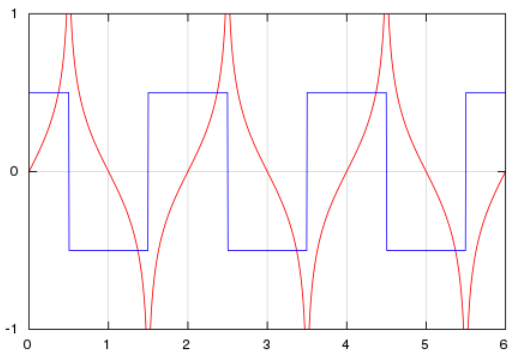
\includegraphics[width=0.6\columnwidth]{Images/hilbert}
\end{center}
